\documentclass[aspectratio=169,10pt]{beamer}
\usepackage[T1]{fontenc}
\usepackage[utf8]{inputenc}
\usepackage{amsmath,amssymb,booktabs,graphicx,tabularx,array}
\usepackage{xcolor}
\usepackage{tikz}
\usetikzlibrary{positioning,arrows.meta}

\definecolor{Ink}{HTML}{06111F}
\definecolor{Panel}{HTML}{10263A}
\definecolor{Line}{HTML}{31506A}
\definecolor{Blue}{HTML}{2563EB}
\definecolor{Cyan}{HTML}{38BDF8}
\definecolor{Amber}{HTML}{F59E0B}
\definecolor{Green}{HTML}{22C55E}
\definecolor{Red}{HTML}{EF4444}
\definecolor{Muted}{HTML}{9CB4C8}
\definecolor{Paper}{HTML}{F8FAFC}

\setbeamercolor{normal text}{fg=Paper,bg=Ink}
\setbeamercolor{frametitle}{fg=Paper,bg=Ink}
\setbeamercolor{title}{fg=Paper,bg=Ink}
\setbeamercolor{block title}{fg=Paper,bg=Panel}
\setbeamercolor{block body}{fg=Paper,bg=Panel}
\setbeamercolor{alerted text}{fg=Amber}
\setbeamerfont{frametitle}{size=\Large,series=\bfseries}
\setbeamerfont{title}{size=\Huge,series=\bfseries}
\setbeamertemplate{navigation symbols}{}
\setbeamertemplate{itemize item}{\color{Amber}$\blacktriangleright$}
\setbeamertemplate{footline}{\hfill\scriptsize\color{Muted}{Probability POV \hspace{1em}\insertframenumber/\inserttotalframenumber}\hspace{1em}\vspace{0.6em}}

\newcommand{\metric}[3]{\begin{block}{#2}\centering{\Huge\bfseries\color{#3}#1}\end{block}}
\newcommand{\smallsource}[1]{\vfill{\tiny\color{Muted}Source: #1}}

\title{Materials Adversarial Learning}
\subtitle{A probability view of attacks, validity, and scientific evidence}
\author{Repository evidence review}
\date{17 October 2026}

\begin{document}

\begin{frame}
  \titlepage
  \vspace{-1em}
  \centering\color{Amber}\large Point estimates become decisions only after uncertainty and validity enter the model.
\end{frame}

\begin{frame}{The probability view changes the central question}
\begin{columns}[T,totalwidth=\textwidth]
\column{0.58\textwidth}
\Large
The useful quantity is not the largest observed drift. It is the probability that a bounded search finds a valid, label-preserving perturbation whose drift exceeds a declared threshold.

\vspace{1em}
\begin{block}{Decision quantity}
\[
P\!\left(V=1,\ L=1,\ D>\tau\mid a,b,x,\mathcal D\right)
\]
\end{block}
\column{0.38\textwidth}
\metric{$n=30$}{sources per benchmark cell}{Cyan}
\metric{$b\in\{5,20,50\}$}{query budgets}{Amber}
\metric{0/22,500}{valid materials generator proposals}{Red}
\end{columns}
\smallsource{results/final/attack\_strategy\_comparison.csv; generator\_quality\_summary.json}
\end{frame}

\begin{frame}{Attack success is a joint event}
\centering
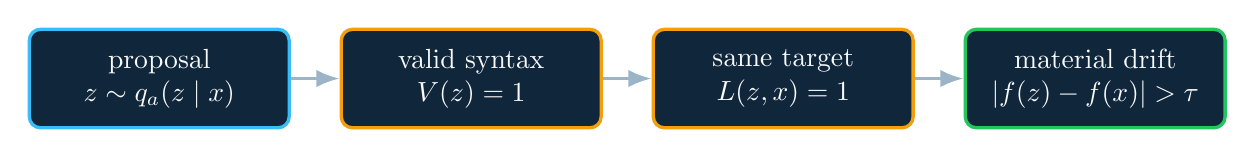
\begin{tikzpicture}[node distance=0.62cm, every node/.style={align=center}]
\node[draw=Cyan,very thick,rounded corners,fill=Panel,text=Paper,minimum width=3.3cm,minimum height=1.25cm] (p) {proposal\\$z\sim q_a(z\mid x)$};
\node[draw=Amber,very thick,rounded corners,fill=Panel,text=Paper,right=of p,minimum width=3.3cm,minimum height=1.25cm] (v) {valid syntax\\$V(z)=1$};
\node[draw=Amber,very thick,rounded corners,fill=Panel,text=Paper,right=of v,minimum width=3.3cm,minimum height=1.25cm] (l) {same target\\$L(z,x)=1$};
\node[draw=Green,very thick,rounded corners,fill=Panel,text=Paper,right=of l,minimum width=3.3cm,minimum height=1.25cm] (d) {material drift\\$|f(z)-f(x)|>\tau$};
\draw[-{Latex},very thick,color=Muted] (p)--(v);
\draw[-{Latex},very thick,color=Muted] (v)--(l);
\draw[-{Latex},very thick,color=Muted] (l)--(d);
\end{tikzpicture}

\vspace{1.2em}
\[
P(S=1)=P(V=1)\,P(L=1\mid V=1)\,P(D>\tau\mid V=1,L=1)
\]

\begin{alertblock}{Current evidence boundary}
The benchmark records syntax validity and prediction drift. It does not establish label preservation for every materials perturbation, so the full success probability remains unidentified.
\end{alertblock}
\end{frame}

\begin{frame}{A Beta posterior makes small-sample uncertainty visible}
For $k$ successes among $n$ sources, use a transparent baseline model:
\[
p_a\sim\mathrm{Beta}(1,1),\qquad p_a\mid k,n\sim\mathrm{Beta}(k+1,n-k+1).
\]

\vspace{0.6em}
\begin{center}
\begin{tabular}{lccc}
\toprule
Bio-cyber, budget 50 & observed & posterior mean & 95\% credible interval\\
\midrule
Evolutionary & 17/30 & 0.562 & [0.391, 0.727]\\
Attribution-High & 17/30 & 0.562 & [0.391, 0.727]\\
MCMC & 14/30 & 0.469 & [0.302, 0.640]\\
Random & 12/30 & 0.406 & [0.245, 0.578]\\
Generative-Trained & 12/30 & 0.406 & [0.245, 0.578]\\
\bottomrule
\end{tabular}
\end{center}

\begin{block}{Interpretation}
The intervals overlap substantially. The evidence supports uncertainty-aware comparisons, not a definitive league table.
\end{block}
\smallsource{Beta(1,1) analysis derived from recorded success counts in attack\_strategy\_comparison.csv}
\end{frame}

\begin{frame}{More queries increase the chance of observing an extreme}
If candidate exceedances were independent with per-query probability $r$, then the chance of at least one success under budget $b$ would be
\[
P(S_b=1)=1-(1-r)^b.
\]

\begin{columns}[T,totalwidth=\textwidth]
\column{0.48\textwidth}
\begin{block}{Why this matters}
Maximum drift rises mechanically with search budget. Comparing methods at unequal budgets confounds search quality with opportunity.
\end{block}
\column{0.48\textwidth}
\begin{block}{Why the formula is only a guide}
MCMC and evolutionary proposals are dependent. Their effective sample size can be far below the raw query count.
\end{block}
\end{columns}

\vspace{0.8em}
The repository's matched budgets of 5, 20, and 50 are therefore essential. Proposal count, target queries, attribution queries, and runtime still need separate accounting.
\end{frame}

\begin{frame}{Validity behaves like a probability gate}
\begin{columns}[T,totalwidth=\textwidth]
\column{0.52\textwidth}
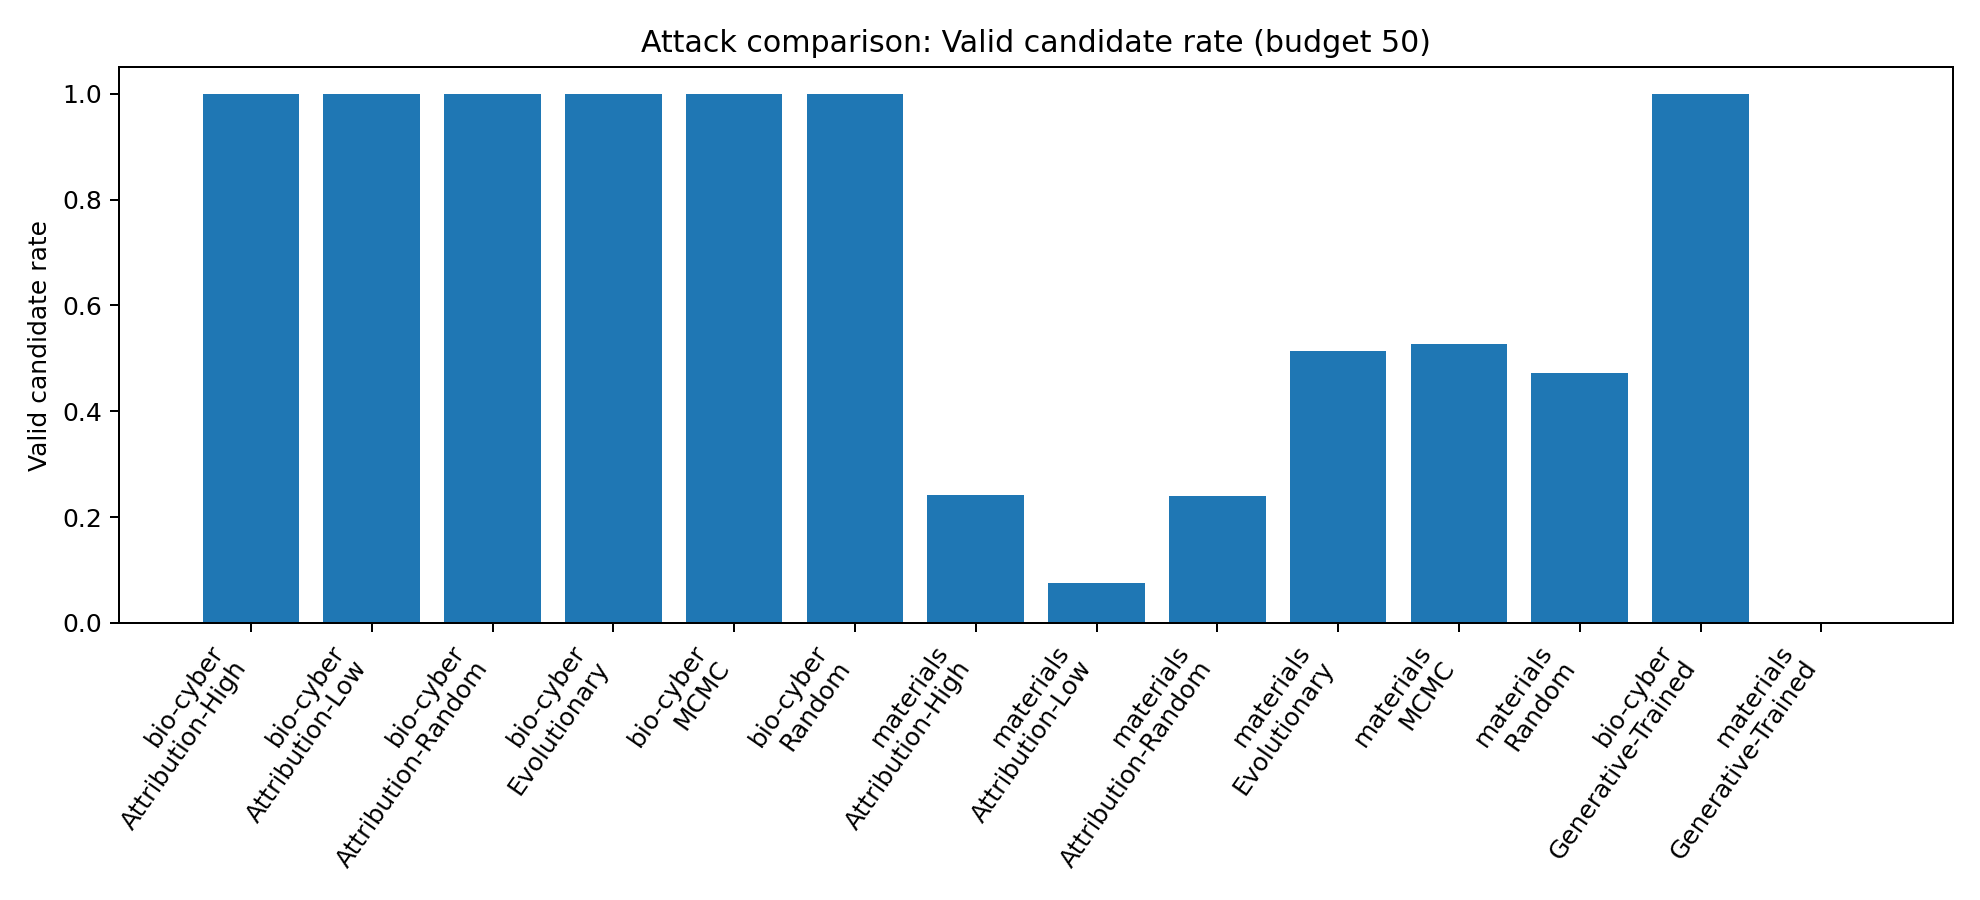
\includegraphics[width=\linewidth]{results/final/figures/attack_strategy_comparison/validity.png}
\column{0.44\textwidth}
\begin{block}{Recorded materials result}
The trained generator produced 0 accepted proposals from 22,500 attempts.
\end{block}

With a uniform prior,
\[
p_V\mid 0,22500\sim\mathrm{Beta}(1,22501).
\]
The 95\% upper credible bound is approximately $1.64\times10^{-4}$.

\vspace{0.6em}
This result says the generator failed the validity gate in this implementation. It does not show that generative attacks are intrinsically weak.
\end{columns}
\smallsource{generator\_quality\_summary.json; validity.png}
\end{frame}

\begin{frame}{Paired tests answer a narrower question than probability of success}
\begin{columns}[T,totalwidth=\textwidth]
\column{0.51\textwidth}
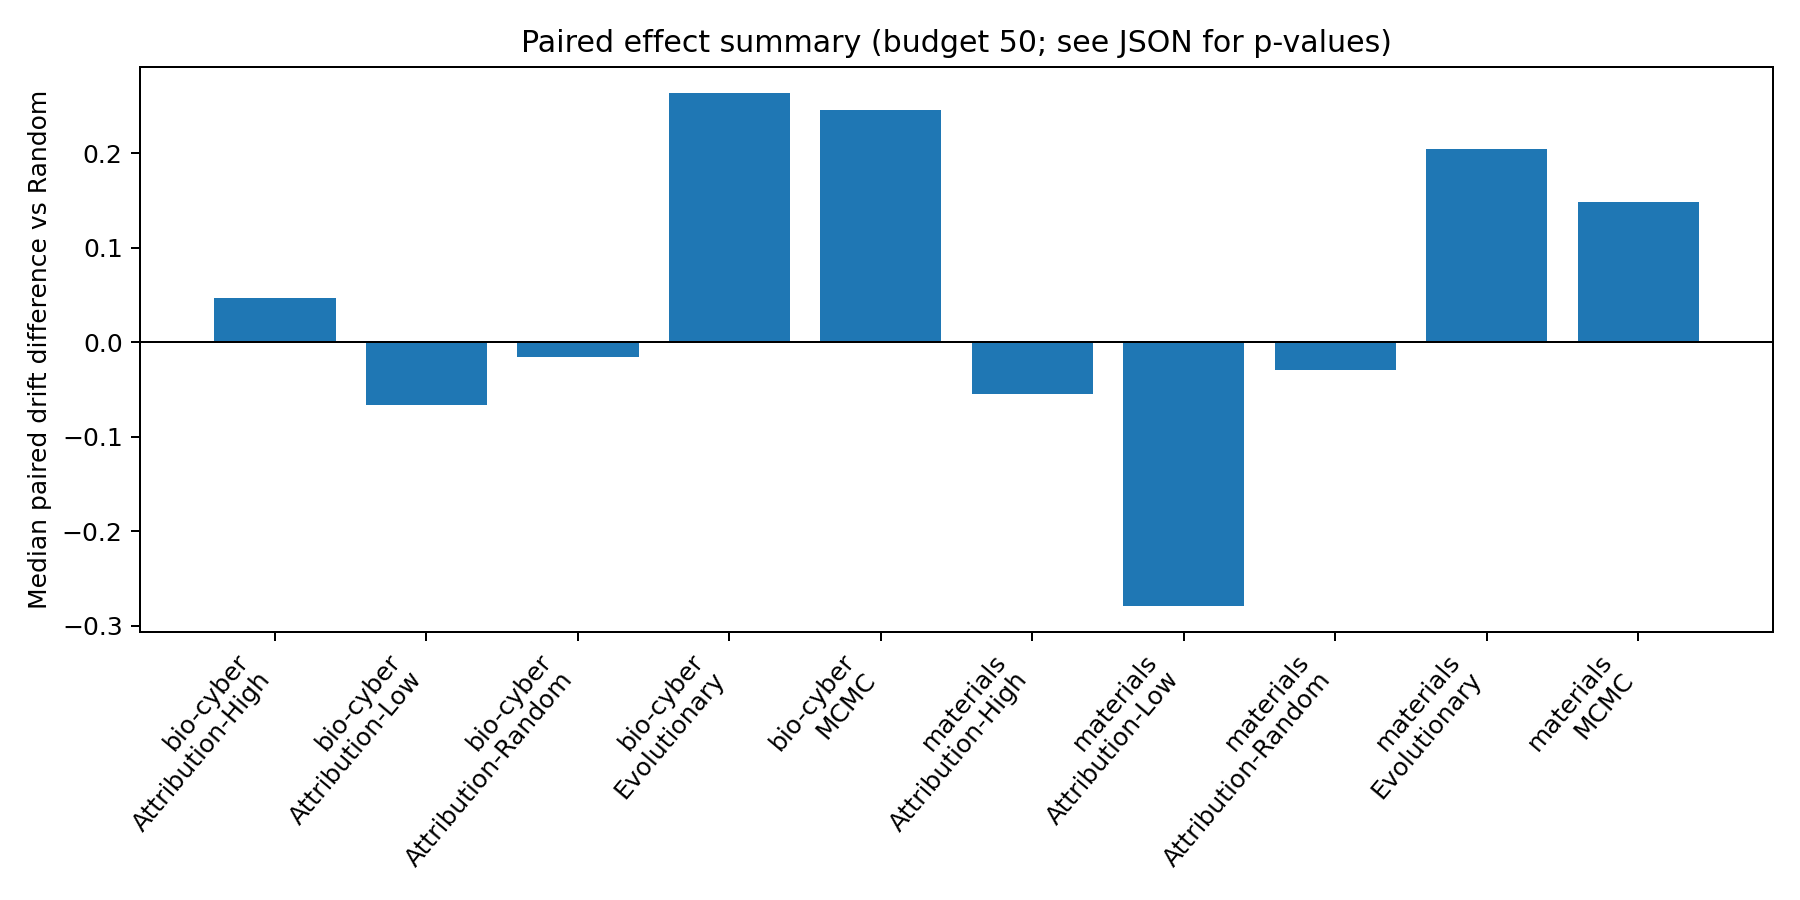
\includegraphics[width=\linewidth]{results/final/figures/attack_strategy_comparison/statistical_comparison.png}
\column{0.45\textwidth}
At budget 50, paired Wilcoxon tests compare drift against Random on the same 30 sources.

\vspace{0.6em}
\begin{tabular}{lrr}
\toprule
Method & Bio median $\Delta$ & Materials median $\Delta$\\
\midrule
Evolutionary & +0.264 & +0.205\\
MCMC & +0.246 & +0.148\\
Attr.-High & +0.047 & -0.055\\
Attr.-Low & -0.066 & -0.280\\
\bottomrule
\end{tabular}

\vspace{0.6em}
Small $p$-values support a distributional difference. They do not give $P(H\mid\mathcal D)$ and do not solve chemical label preservation.
\end{columns}
\smallsource{statistical\_results.json; two-sided paired Wilcoxon tests}
\end{frame}

\begin{frame}{Search trajectories are stochastic objects}
\centering
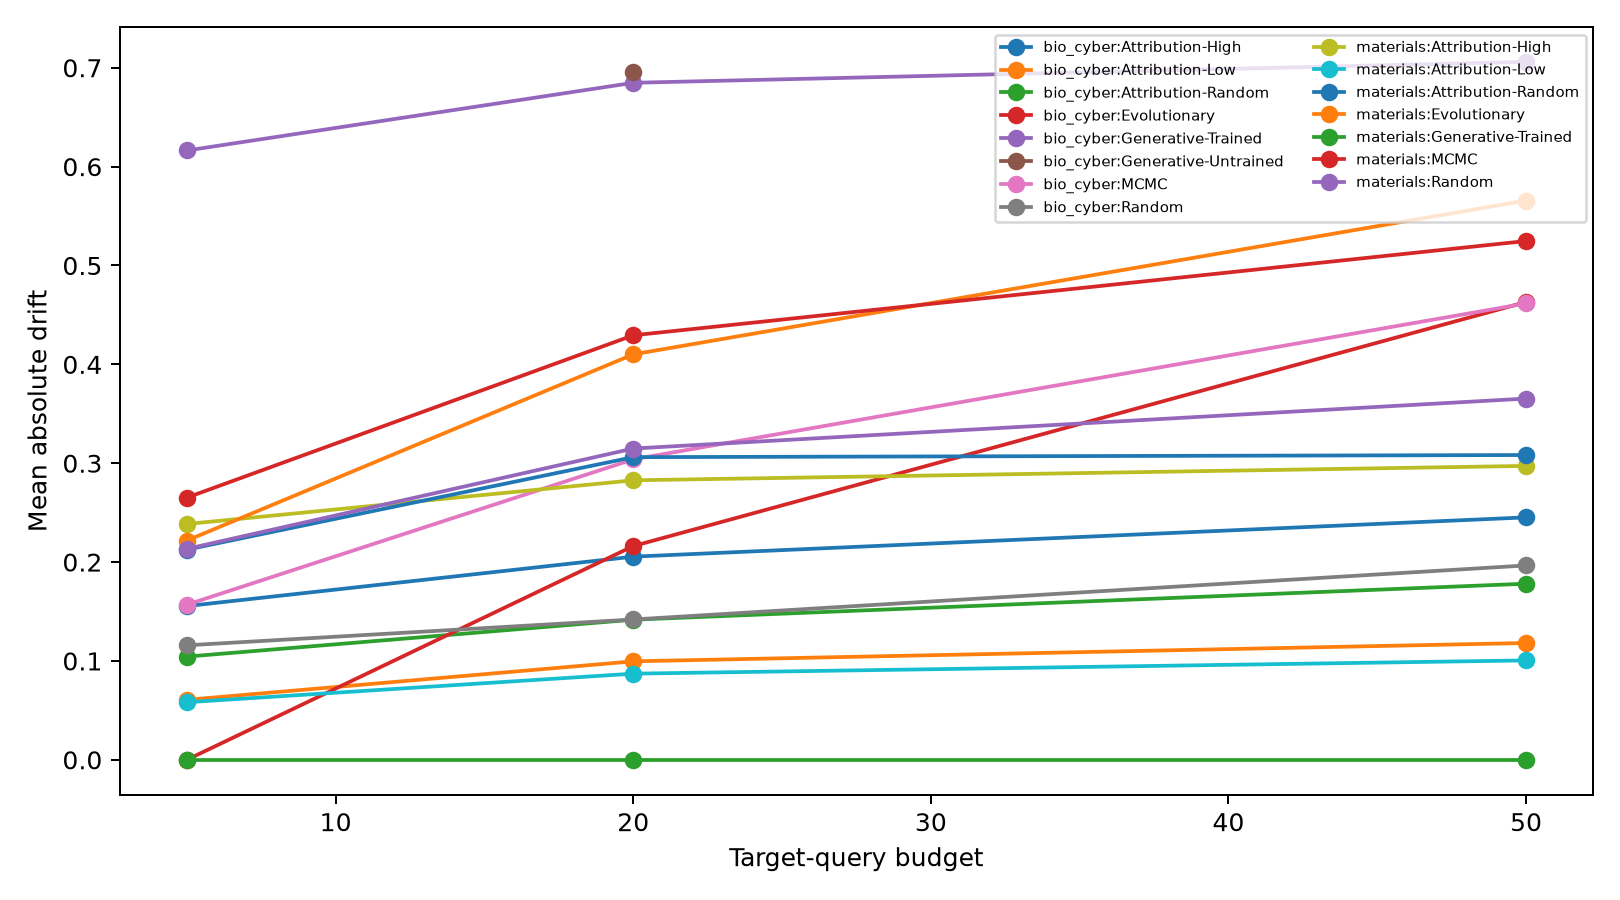
\includegraphics[width=0.82\linewidth]{results/final/figures/attack_strategy_comparison/budget_trajectories.png}

\vspace{0.35em}
\begin{block}{Probability interpretation}
Each curve summarizes a random search path. A robust comparison needs variation across sources and seeds, plus the probability of reaching a useful threshold by a fixed budget.
\end{block}
\smallsource{budget\_trajectories.png; current comparison uses seed 42 in the summary table}
\end{frame}

\begin{frame}{Selection creates optimism unless evaluation stays sealed}
\begin{columns}[T,totalwidth=\textwidth]
\column{0.55\textwidth}
\begin{block}{Recommended hierarchy}
\[
\begin{aligned}
\theta_{a,d,b}&=\text{latent attack effect},\\
y_{i,a,d,b}&\sim F(\theta_{a,d,b},\sigma_{d}),\\
\theta_{a,d,b}&\sim\mathcal N(\mu_a+\delta_d+\gamma_b,\tau^2).
\end{aligned}
\]
Partial pooling reduces noisy rankings across domains and budgets.
\end{block}
\column{0.41\textwidth}
\begin{itemize}
\item Choose thresholds and hyperparameters on validation data.
\item Freeze attack banks before final model comparison.
\item Open the test set once for the declared analysis.
\item Report every attempted family, including blocked and rejected methods.
\end{itemize}
\end{columns}

\begin{alertblock}{Repository boundary}
Phase 6 defense selection was previously incomplete. This deck does not convert progress artifacts into final defense evidence.
\end{alertblock}
\end{frame}

\begin{frame}{A decision rule should combine effect, validity, and cost}
For a deployment or publication decision, define utility explicitly:
\[
U(a)=P(S=1\mid a,b,\mathcal D)\,B_{\mathrm{finding}}
-C_{\mathrm{queries}}(a)-C_{\mathrm{runtime}}(a)-C_{\mathrm{invalid}}(a).
\]

\begin{columns}[T,totalwidth=\textwidth]
\column{0.48\textwidth}
\begin{block}{Promote a method when}
Posterior probability of a practically important advantage exceeds a preregistered threshold and validity evidence passes its gate.
\end{block}
\column{0.48\textwidth}
\begin{block}{Keep a method exploratory when}
Evidence depends on one seed, label preservation is unverified, or external credentials and compute block the planned comparison.
\end{block}
\end{columns}

\vspace{0.7em}
Suggested reporting target: $P(\Delta>\delta_{\min}\mid\mathcal D)$, not only $p<0.05$.
\end{frame}

\begin{frame}{What the current evidence supports}
\begin{columns}[T,totalwidth=\textwidth]
\column{0.31\textwidth}
\metric{Supported}{Budget changes observed drift and success frequency}{Green}
\column{0.31\textwidth}
\metric{Supported}{Several paired drift distributions differ from Random}{Green}
\column{0.31\textwidth}
\metric{Supported}{The materials generator failed its validity gate}{Red}
\end{columns}

\vspace{0.8em}
\begin{alertblock}{Not yet identified}
The probability of a chemically label-preserving attack, cross-seed stability of rankings, and a final defended-model benefit on a sealed test set.
\end{alertblock}

\smallsource{final comparison artifacts plus repository evidence-status notes}
\end{frame}

\begin{frame}{Next experiment: estimate probabilities that answer decisions}
\begin{enumerate}
\item Declare a domain-specific drift threshold $\tau$ and minimum useful advantage $\delta_{\min}$.
\item Run multiple seeds for every source, method, and matched query budget.
\item Add an independent label-preservation oracle or mark the event unknown.
\item Fit a hierarchical model across sources, budgets, and domains.
\item Report posterior intervals, threshold-crossing probabilities, calibration, and cost.
\item Preserve blocked, incomplete, and rejected methods in the final comparison table.
\end{enumerate}

\vspace{0.8em}
\begin{block}{Bottom line}
Probability turns the project from a collection of maximum drifts into a calibrated statement about how often a valid attack works, under what budget, and with what uncertainty.
\end{block}
\end{frame}

\end{document}
